%%%%%%%%%%%%%%%%%%%%%%%%%%%%%%%%%%%%%%%%%
% Beamer Presentation
% LaTeX Template
% Version 1.0 (10/11/12)
%
% This template has been downloaded from:
% http://www.LaTeXTemplates.com
%
% License:
% CC BY-NC-SA 3.0 (http://creativecommons.org/licenses/by-nc-sa/3.0/)
%
%%%%%%%%%%%%%%%%%%%%%%%%%%%%%%%%%%%%%%%%%

%----------------------------------------------------------------------------------------
%	PACKAGES AND THEMES
%----------------------------------------------------------------------------------------

\documentclass[aspectratio=169]{beamer}
\usepackage{listings}

\usepackage{color}
\usepackage{booktabs}
\usepackage{enumitem}

\definecolor{mygray}{rgb}{0.4,0.4,0.4}
\definecolor{myorange}{rgb}{1.0,0.4,0}

\lstset{
basicstyle=\tiny\sffamily\color{black},
commentstyle=\color{mygray},
frame=single,
keywordstyle=\color{blue},
showspaces=false,
showstringspaces=false,
stringstyle=\color{myorange},
tabsize=2,
language=C++
}


\mode<presentation> {

% The Beamer class comes with a number of default slide themes
% which change the colors and layouts of slides. Below this is a list
% of all the themes, uncomment each in turn to see what they look like.

%\usetheme{default}
%\usetheme{AnnArbor}
%\usetheme{Antibes}
%\usetheme{Bergen}
%\usetheme{Berkeley}
%\usetheme{Berlin}
%\usetheme{Boadilla}
\usetheme{CambridgeUS}
%\usetheme{Copenhagen}
%\usetheme{Darmstadt}
%\usetheme{Dresden}
%\usetheme{Frankfurt}
%\usetheme{Goettingen}
%\usetheme{Hannover}
%\usetheme{Ilmenau}
%\usetheme{JuanLesPins}
%\usetheme{Luebeck}
%\usetheme{Madrid}
%\usetheme{Malmoe}
%\usetheme{Marburg}
%\usetheme{Montpellier}
%\usetheme{PaloAlto}
%\usetheme{Pittsburgh}
%\usetheme{Rochester}
%\usetheme{Singapore}
%\usetheme{Szeged}
%\usetheme{Warsaw}

% As well as themes, the Beamer class has a number of color themes
% for any slide theme. Uncomment each of these in turn to see how it
% changes the colors of your current slide theme.

%\usecolortheme{albatross}
%\usecolortheme{beaver}
%\usecolortheme{beetle}
%\usecolortheme{crane}
%\usecolortheme{dolphin}
%\usecolortheme{dove}
%\usecolortheme{fly}
%\usecolortheme{lily}
%\usecolortheme{orchid}
%\usecolortheme{rose}
%\usecolortheme{seagull}
%\usecolortheme{seahorse}
%\usecolortheme{whale}
%\usecolortheme{wolverine}

%\setbeamertemplate{footline} % To remove the footer line in all slides uncomment this line
%\setbeamertemplate{footline}[page number] % To replace the footer line in all slides with a simple slide count uncomment this line

\setbeamertemplate{navigation symbols}{} % To remove the navigation symbols from the bottom of all slides uncomment this line
}
\setbeamercovered{transparent}
\setbeamersize{text margin left=30pt,text margin right=30pt} 


\usepackage[utf8]{inputenc}
\usepackage{graphicx} % Allows including images
\usepackage{booktabs} % Allows the use of \toprule, \midrule and \bottomrule in tables

\setitemize{label=\usebeamerfont*{itemize item}%
  \usebeamercolor[fg]{itemize item}
  \usebeamertemplate{itemize item}}

\setlist[description]{leftmargin=\parindent, labelindent=\parindent}

%----------------------------------------------------------------------------------------
%	TITLE PAGE
%----------------------------------------------------------------------------------------

\title[Randomness Testing Toolkit]{The automated testing of randomness with multiple statistical batteries} % The short title appears at the bottom of every slide, the full title is only on the title page

\author[lubomir.obratil@gmail.com]{Ľubomír Obrátil\\lubomir.obratil@gmail.com} % Your name
\date{22. 6. 2017} % Date, can be changed to a custom date

% Eliminates margins
\def\nomar{\list{}{\rightmargin-30pt \leftmargin-30pt}\item[]}
\let\endnomar=\endlist

\usepackage{makecell}
\usepackage{xcolor, colortbl}

\renewcommand\theadfont{\bfseries}

\begin{document}

\begin{frame}
\titlepage % Print the title page as the first slide
\end{frame}

%----------------------------------------------------------------------------------------
%	PRESENTATION SLIDES
%----------------------------------------------------------------------------------------
\begin{frame}
\frametitle{Presentation structure}

\begin{itemize}
\item RTT implementation -- program and service, deployed on MetaCentrum
\item Brief intro into statistical testing -- battery, test, hypothesis, partial results, false positives/negatives
\item Baseline experiment -- default behaviour of the batteries, what is the rate of false negative tests, find the thresholds, use it in the subsequent testing
\item Security margins experiment -- compare to EACirc (?), compare strength of individual batteries in RTT, detect discrepancies
\item Dieharder experiment -- distribution of the partial results, assumed uniformity, however different results obtained, show how much.
\end{itemize}
\end{frame}

%%%%%%%%%%%%%%%%%%%%%%%%%%%%%%%%
% Statistical testing overview %
%%%%%%%%%%%%%%%%%%%%%%%%%%%%%%%%
\begin{frame}
\frametitle{Statistical testing of randomness}

\begin{description}
\item[Statistical battery] \hfill \\
Software with purpose of detecting biases in data stream; collection of statistical tests.
\item[Statistical test] \hfill \\
Single unit in statistical battery, checks some property of the data; e.g. longest
uninterrupted stream of ones.
\item[Null hypothesis -- $H_0$] \hfill \\
Null hypothesis stating that the tested data were produced by a true random number
generator.
\item[False positive (Type I error)] \hfill \\
Happens when $H_0$ holds true but it is rejected -- truly random stream is evaluated as non random. We assume that for random data the p-values have an uniform distribution -- probability of Type I error is $\alpha$.

\item[False negative (Type II error)] \hfill \\
Happens when $H_0$ is false but it is not rejected -- biased stream is evaluated as random.
\end{description}

\end{frame}


%%%%%%%%%%%%%%%%%%%%%%%%%%%%%%%%%%%%%%%
% Randomness Testing Toolkit overview %
%%%%%%%%%%%%%%%%%%%%%%%%%%%%%%%%%%%%%%%
\begin{frame}
\frametitle{Randomness Testing Toolkit -- motivation}
\begin{Huge}
TODO
\end{Huge}
\end{frame}

\begin{frame}
\frametitle{Randomness Testing Toolkit -- local interface}
\begin{nomar}
\centering
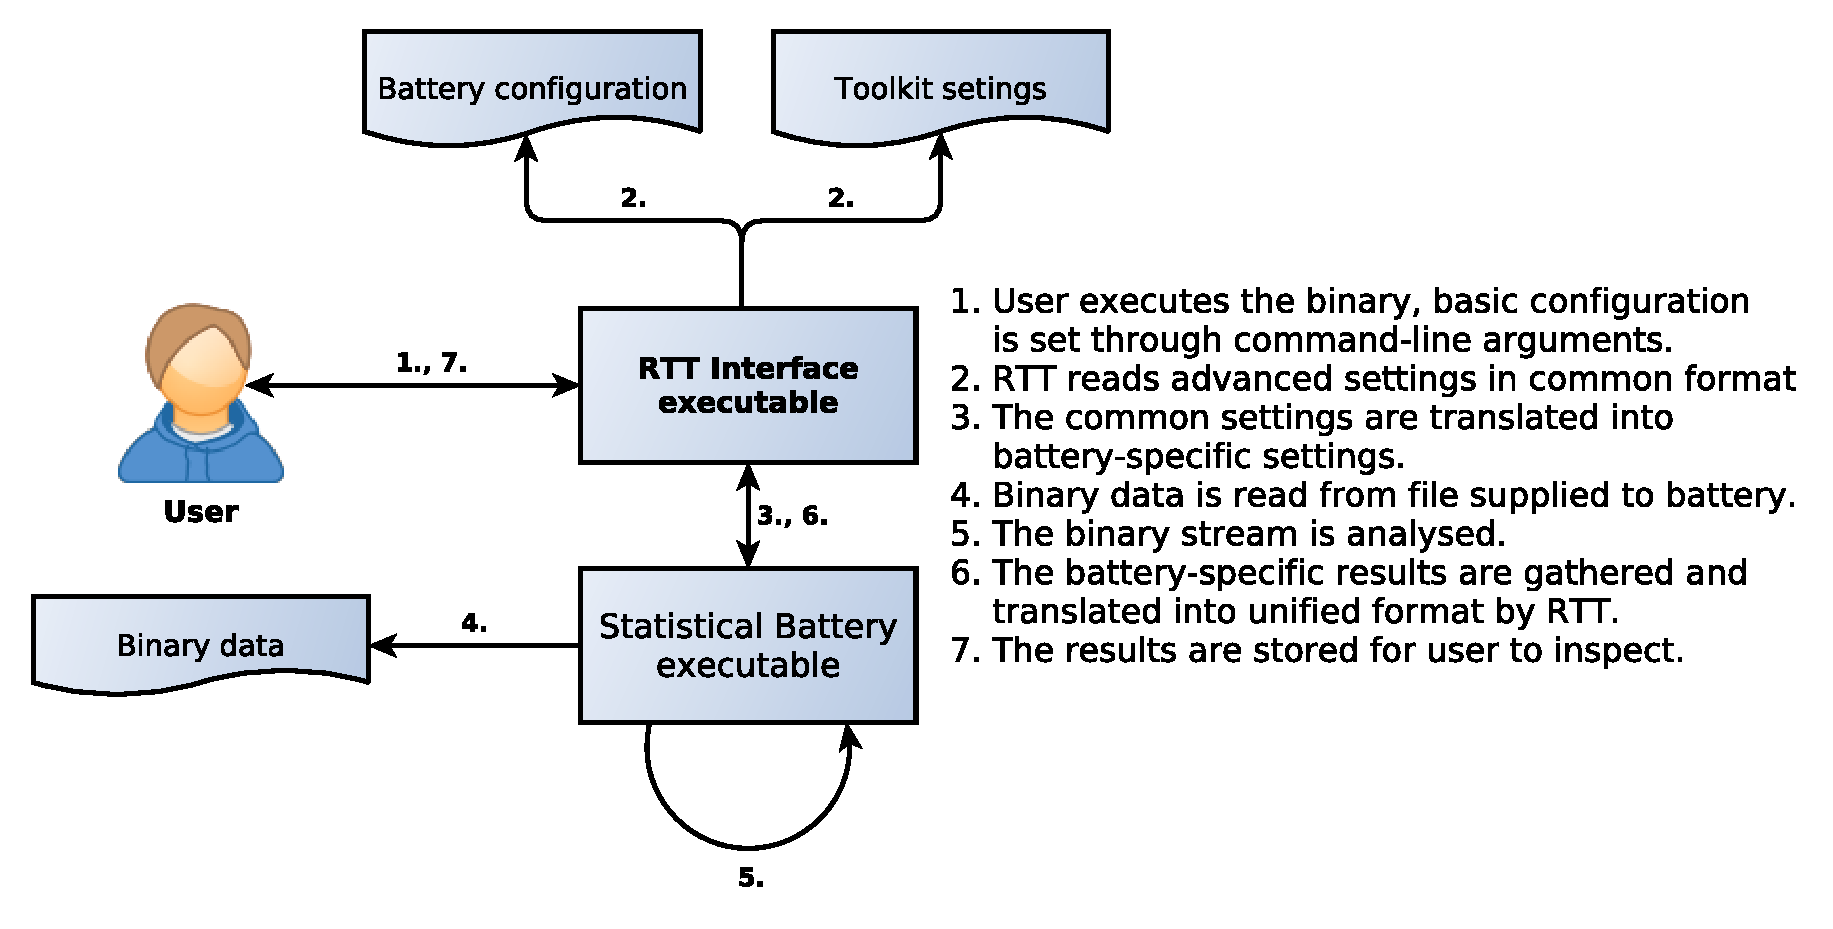
\includegraphics[width=\textwidth]{figures/local-rtt-workflow.pdf} 
\end{nomar}
\end{frame}

\begin{frame}
\frametitle{Randomness Testing Toolkit -- web service}
\begin{nomar}
\centering
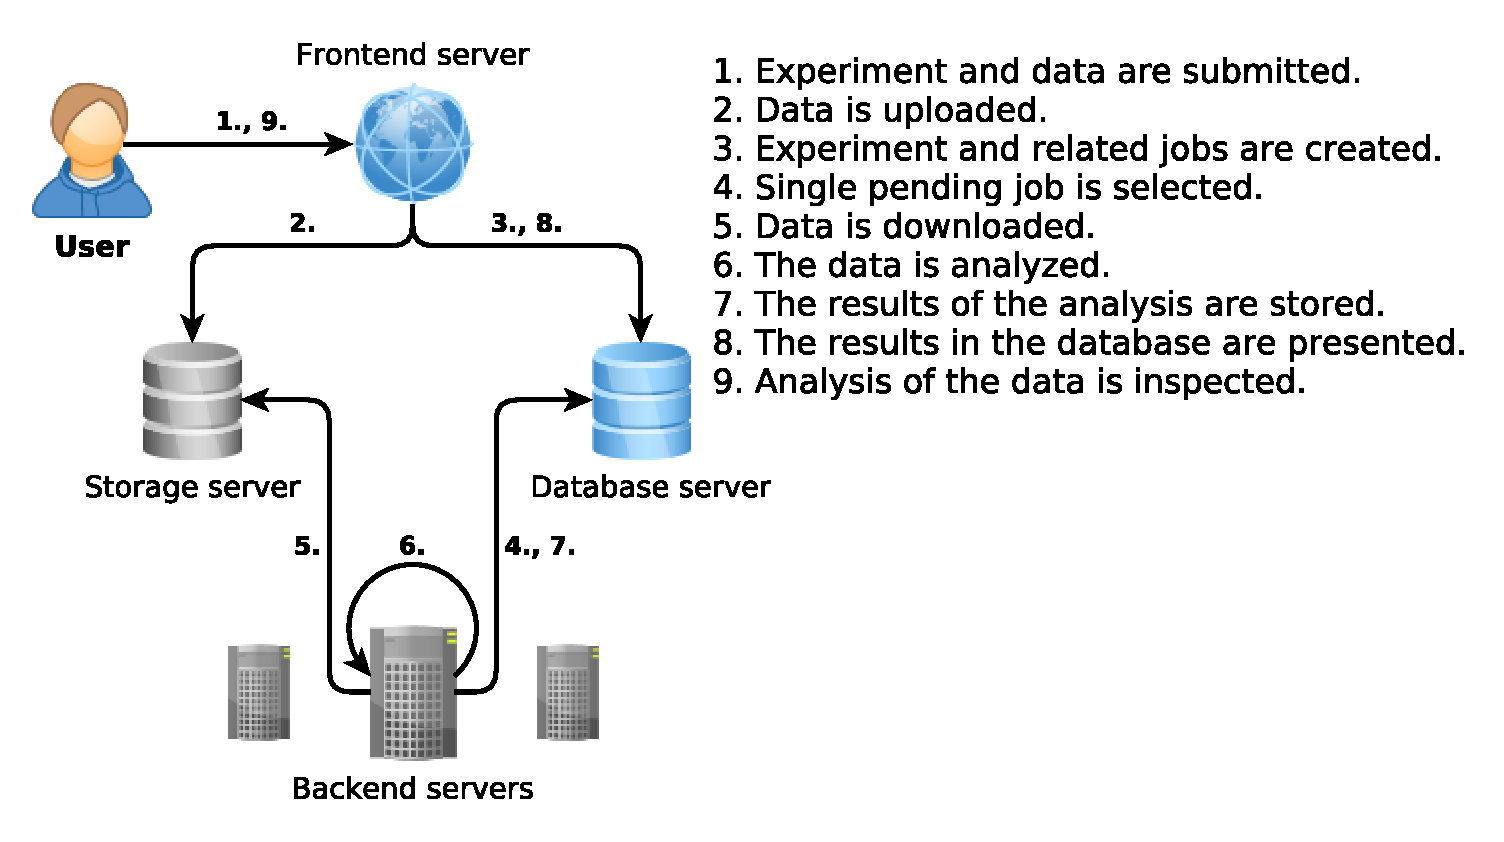
\includegraphics[width=.9\textwidth]{figures/rtt-ecosystem.pdf} 
\end{nomar}
\end{frame}

%%%%%%%%%%%%%%%%%%%%%%%%%%%
% Experiments -- baseline %
%%%%%%%%%%%%%%%%%%%%%%%%%%%

%%%%%%%%%%%%%%%%%%%%%%%%%%%%%%%%%%%
% Experiments -- security margins %
%%%%%%%%%%%%%%%%%%%%%%%%%%%%%%%%%%%

%%%%%%%%%%%%%%%%%%%%%%%%%%%%%%%%%%%
% Experiments -- faulty Dieharder %
%%%%%%%%%%%%%%%%%%%%%%%%%%%%%%%%%%%

\begin{frame}
\frametitle{Talk overview}
\begin{itemize}
\item \textbf{Randomness Testing Toolkit project}
\begin{itemize}
\item Developed framework for randomness testing
\end{itemize}
\item \textbf{Introduction to statistical testing}
\begin{itemize}
\item Theory behind the statistical tests
\end{itemize} 
\item \textbf{Experiments done with RTT}
\begin{itemize}
\item Baseline experiment
\item Analysis of popular crypto functions
\item Dieharder outputs inspection
\end{itemize}
\end{itemize}
\end{frame}

\begin{frame}
\frametitle{Randomness Testing Toolkit}

\begin{description}
\item[Motivation] \hfill \\
\begin{itemize}
\item Randomness testing used for benchmarking of the research tools developed in CRoCS. TODO: Add another reason, make it easy.
\item Most of the existing statistical batteries are neither intuitive nor trivial to use.
\item Inconsistent results among researchers.
\end{itemize}

\vspace{.5cm}

\item[Randomness Testing Toolkit] \hfill \\
\begin{itemize}
\item Project aiming to provide easy, fast and consistent randomness testing.
\item Inclusion of multiple statistical batteries -- NIST STS, Dieharder, TestU01.
\item Available as a standalone executable or as a service.
\end{itemize}
\end{description}

\end{frame}

\begin{frame}
\frametitle{Randomness Testing Toolkit}

\begin{Huge}
Here goes the figure...
\end{Huge}

\end{frame}

\begin{frame}
\frametitle{Statistical testing -- 1/3}

\begin{description}
\item[Statistical battery] \hfill \\ 
Software with purpose of detecting biases in data stream; collection of statistical tests.
\item[Statistical test] \hfill \\
Single unit in statistical battery, checks some property of the data; e.g. longest uninterrupted stream of ones.

\vspace{.3cm}

\item[Statistical test results -- REWORK] \hfill \\
\begin{itemize}
\item Single test is repeated multiple times, resulting in multiple first-level p-values.
\item First-level p-values are processed by arbitrary statistical algorithm -- the result is second-level p-value or statistic; e.g. Kolmogorov-Smirnov test for uniformity.
\item Single test can produce multiple statistics (subtests, variations in test parameters, multiple uniformity tests, etc...).
\end{itemize}
\end{description}

\end{frame}

\begin{frame}
\frametitle{Statistical testing -- 2/3}

\begin{description}
\item[Hypothesis $H_0$] \hfill \\
Null hypothesis stating that the tested data were produced by a true random number generator.
\item[p-value] \hfill \\
P-value represents the probability that the $H_0$ holds true.
\item[Significance level $\alpha$] \hfill \\
If p-value is lesser than $\alpha$ then the result is significant and $H_0$ is rejected. If the p-value of a test if lesser than $\alpha$ we consider the test failed.
\item[False positive (Type I error)] \hfill \\
Happens when $H_0$ holds true but it is rejected -- truly random stream is evaluated as non random. We assume that for random data the p-values have an uniform distribution -- probability of Type I error is $\alpha$.
\item[False negative (Type II error)] \hfill \\
Happens when $H_0$ is false but it is not rejected -- biased stream is evaluated as random.
\end{description}

\end{frame}

\begin{frame}
\frametitle{Statistical testing -- 3/3}

\begin{figure}
\begin{nomar}
\centering
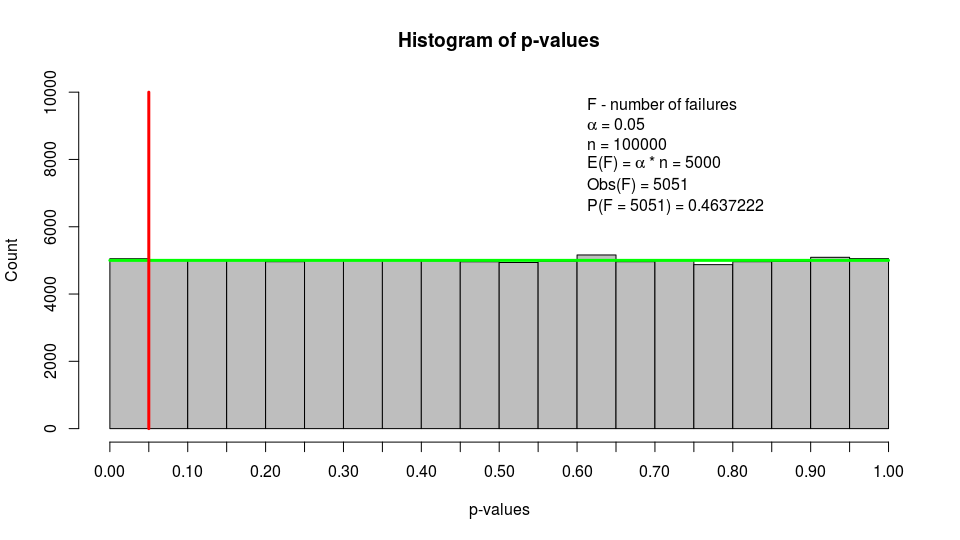
\includegraphics[width=.8\paperwidth]{figures/single-fails-4.png} 
\end{nomar}
\end{figure}

\end{frame}

\begin{frame}
\frametitle{Overview of the experiments}

\begin{description}
\item[Baseline experiment] \hfill \\
\begin{itemize}
\item Discovering failure rates of the batteries
\item Finding the bound of test failure count in a battery
\end{itemize}
\vspace{.2cm}
\item[Usable testbed analysis] \hfill \\
\begin{itemize}
\item Analyse outputs of well-known cryptographic algorithms (AES, DES, RC4, etc.)
\item Observe the security margins of the algorithms
\item Compare the results to other approach in CRoCS
\end{itemize}
\vspace{.2cm}
\item[Analysis of Dieharder] \hfill \\
\begin{itemize}
\item Examine behavior of Dieharder battery during truly random data analysis
\item Analyse the distribution of the results
\end{itemize}
\end{description}

\end{frame}

\begin{frame}
\frametitle{Baseline experiment -- 1/4}

\begin{description}
\item[Analysis of 8TB of quantum random data] \hfill \\
\begin{itemize}
\item Data split into 1000 blocks -- each battery executed on every block
\item Sample size was 1000 trials.
\end{itemize}
\vspace{.2cm}
\item[Test failure observation] \hfill \\
\begin{itemize}
\item Raw second-level p-values -- assuming that p-values are independent.
\begin{itemize}
\item Single p-value will fail with probability $\alpha$
\item Out of $n$ p-values, $x$ will fail with probability $P(F=x) = { n \choose x } * \alpha^x * (1-\alpha)^{n-x}$
\end{itemize}
\item Corrected p-values -- likely-dependent p-values grouped together
\begin{itemize}
\item Products of a single test treated as a single result.
\item Each group of $n$ p-values has new corrected (partial) $\alpha_0 = 1 - (1 - \alpha)^{\frac{1}{n}}$
\item If any p-value in the group with $\alpha_0$ has lesser value than the $\alpha_0$, the entire group is treated as a failed test.
\end{itemize}
\end{itemize}
\end{description}

\end{frame}

\begin{frame}
\frametitle{Baseline experiment -- 2/4}
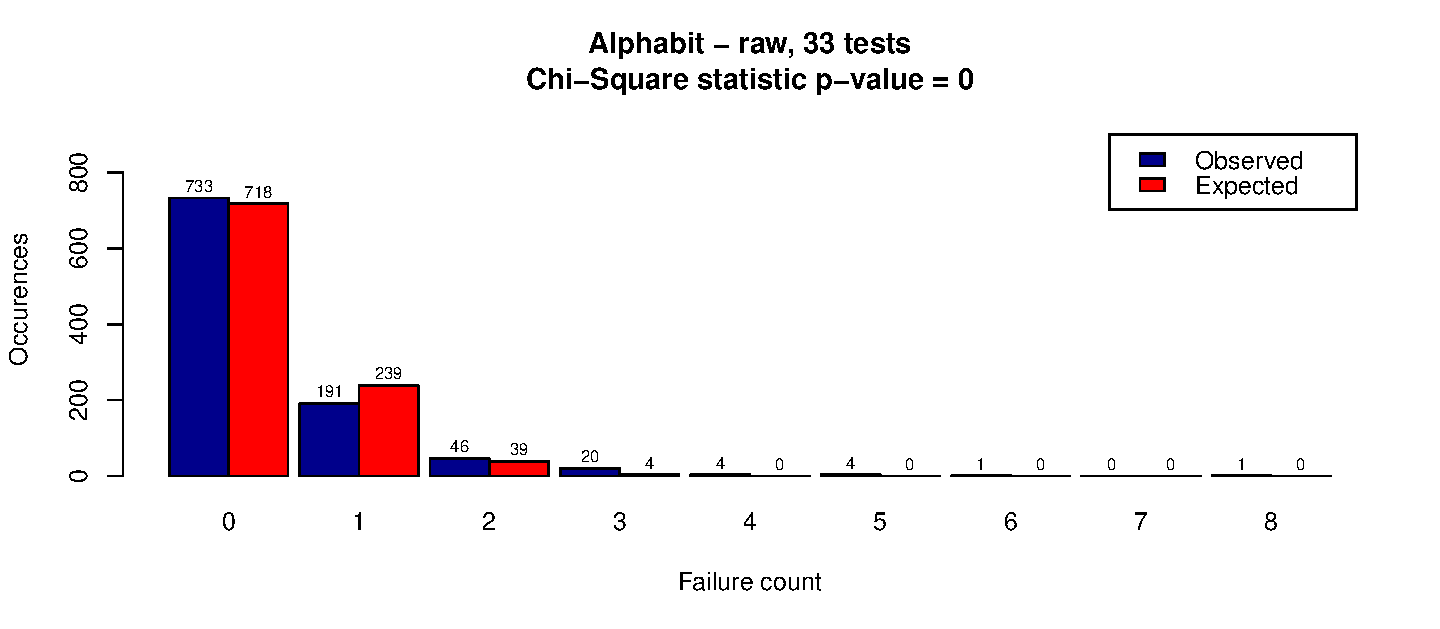
\includegraphics[width=15cm, height=7cm]{figures/corrected_vs_raw/alphabit-raw.pdf} 
\begin{figure}
\begin{nomar}
\centering
\end{nomar}
\end{figure}

\end{frame}

\begin{frame}
\frametitle{Baseline experiment -- 3/4}
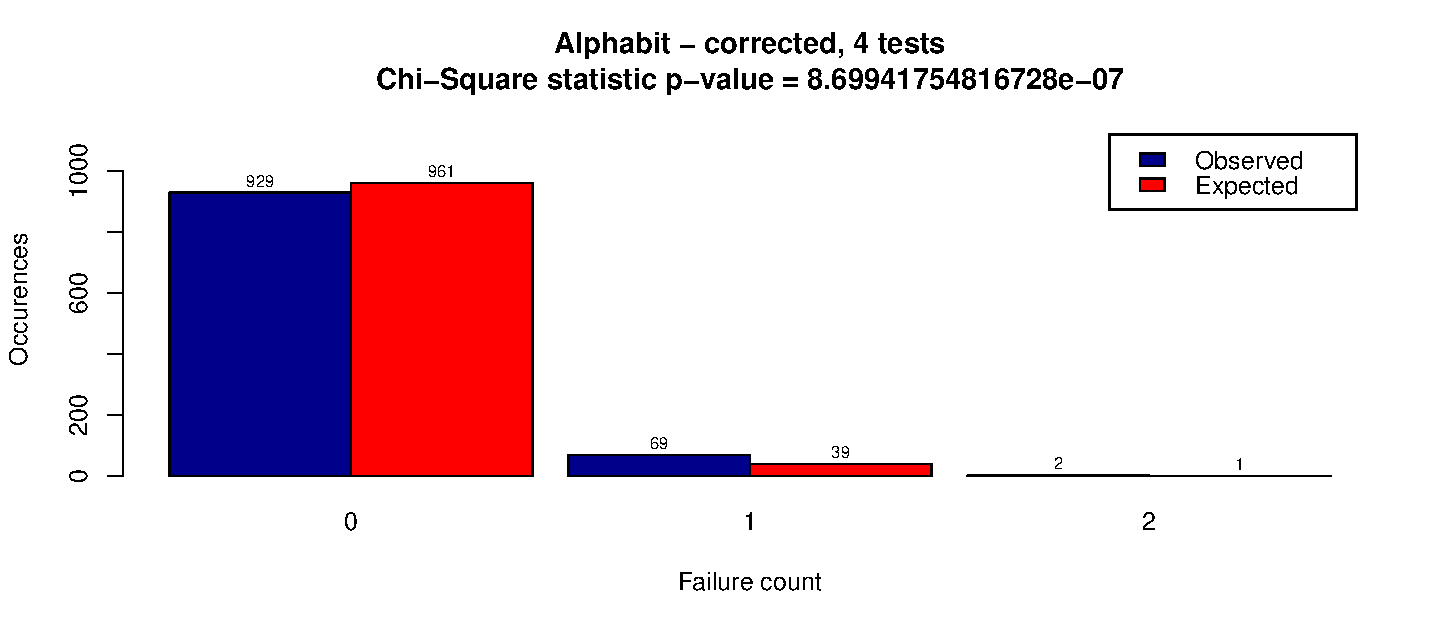
\includegraphics[width=15cm, height=7cm]{figures/corrected_vs_raw/alphabit-corrected.pdf} 
\begin{figure}
\begin{nomar}
\centering
\end{nomar}
\end{figure}

\end{frame}

\begin{frame}
\frametitle{Baseline experiment -- 4/4}

\begin{description}
\item[Analysis result assessment] \hfill \\
\begin{itemize}
\item Result of data analysis is assessed based on the number of failed corrected tests in the battery.
\item $P(X=F) < 0.001$ -- the analysed data is not considered random
\end{itemize}
\item[Summary] \hfill \\
\begin{table}
\begin{nomar}
\centering
\begin{tabular}{l || r | r | r}
\textbf{Battery name} & \textbf{Raw} $\chi^2$ & \textbf{Corrected} $\chi^2$ & \textbf{Fail count bound} \\ \hline \hline
Dieharder            & 4.3e-17          & \textbf{0.50427}  & 3/27 \\ 
NIST STS             & \textbf{0.02975} & 5.5e-09           & 2/15 \\ 
TU01 Small Crush     & \textbf{0.72575} & 0.15814           & 2/10 \\ 
TU01 Crush           & 3.6e-15          & \textbf{0.00707}  & 3/32 \\ 
TU01 Rabbit          & \textbf{4.9e-22} & 1.4e-23           & 2/16 \\ 
TU01 Alphabit        & 0.00000          & \textbf{8.6e-07}  & 1/4 \\ 
TU01 Block Alphabit  & 0.00000          & \textbf{1.4e-101} & 1/4 \\
\end{tabular}
\end{nomar}
\end{table}
\end{description}

\end{frame}

\begin{frame}
\frametitle{Usable testbed analysis -- 1/3}

\begin{description}
\item[Analysed algorithms] \hfill \\
\begin{itemize}
\item In total, 72 different data streams were analysed.
\item The data streams were outputs from 16 distinct round-reduced cryptographic algorithms.
\item The algorithms were chosed based on their popularity (AES, DES, RC4, ...) or their success in crypto competitions eSTREAM and SHA3 (Rabbit, Keccak, Gr\o stl, ...).
\end{itemize}
\vspace{.2cm}
\item[Analysis conditions] \hfill \\
\begin{itemize}
\item Each datastream was 8GB long.
\item The conditions of analysis were same as in the previous experiment.
\item The interpretation of the result was based on the results of the baseline experiment.
\end{itemize}
\end{description}

\end{frame}

\begin{frame}
\frametitle{Usable testbed analysis -- 2/3}

\begin{table}
\begin{nomar}
\centering

\scalebox{0.75} {
\begin{tabular}{l || r | r | r }
\textbf{Algorithm} & \thead{Biased round \\ RTT} & \thead{Biased round \\ EACirc} & \textbf{Security Margin} \\ \hline \hline
AES        & 3                          & 3  & 7 -- 70\% \\
BLAKE      & 1                          & 1  & 15 -- 93.7\% \\
Grain      & \cellcolor{green!40}6*     & 2  & 7 -- 53.8\% \\
Gr\o stl   & 2                          & 2  & 12 -- 85.7\% \\
HC-128     & --                         & -- & 0 -- 100\% \\
JH         & 6                          & 6  & 36 -- 85.7\% \\
Keccak     & \cellcolor{green!40}3      & 2  & 21 -- 87.5\% \\
MD6        & \cellcolor{green!40}10*    & 8  & 94 -- 90.3\% \\
Rabbit     & \cellcolor{green!40}4*     & 0  & \cellcolor{red!40}0 -- 0\% \\
RC4        & \cellcolor{green!40}0*     & -- & \cellcolor{red!40}0 -- 0\% \\
Salsa20    & 2                          & 2  & 18 -- 90\% \\
SINGLE-DES & \cellcolor{green!40}5      & 4  & 11 -- 68.7\% \\
Skein      & \cellcolor{green!40}4      & 3  & 68 -- 94.4\% \\
SOSEMANUK  & 4                          & 4  & 21 -- 84\% \\
TEA        & \cellcolor{green!40}5      & 4  & 27 -- 84.3\% \\
TRIPLE-DES & \cellcolor{green!40}3      & 2  & 13 -- 81.2\% \\
\end{tabular}
}
\end{nomar}
\end{table}

\end{frame}

\begin{frame}
\frametitle{Usable testbed analysis -- 3/3}

\begin{description}
\item[Notable results] \hfill \\
\begin{itemize}
\item \textbf{Grain} -- Tests smarsa\_MatrixRank and scomp\_LinearComp (Crush, Rabbit) will fail in 3, 4, 5 and 6-round configuration.
\item \textbf{MD6} -- Tests smarsa\_MatrixRank and sspectral\_Fourier3 (Crush, Rabbit) will fail in 9 and 10-round configuration.
\item \textbf{Rabbit} -- Tests sstring\_HammingIndep and sstring\_PeriodsInStrings (Crush, Rabbit, Alphabit, Block Alphabit) will fail in \textbf{full} configuration.
\item \textbf{RC4} -- Tests sknuth\_SimpPoker and sknuth\_Gap (Crush) will fail in \textbf{full} configuration.
\end{itemize}
\end{description}

\end{frame}

\begin{frame}
\frametitle{Analysis of Dieharder -- 1/2}

\begin{description}
\item[Analysed data] \hfill \\
\begin{itemize}
\item 8TB of quantum random data processed continuously by the tests - single application of a test to a data stream will yield single first-level p-value
\item Uniformity of the first level p-values was analysed.
\item The p-values should be uniformly distributed on the interval $<0,1>$.
\item Total of 110 sets of p-values (single set per raw, uncorrected test) was inspected.
\item Each set had a different size -- usually between 1 to 2 millions of p-values per set.
\end{itemize}
\vspace{.2cm}
\item[Experiment results] \hfill \\
\begin{itemize}
\item Out of 110 p-value sets, 39 sets were not uniformly distributed
\item Chi-Square ($\chi^2$) statistic used for uniformity testing. When the p-value of the statistic was less than 0.001, the inspected set was considered non-uniform.
\item Flawed non-uniform distributions can have impact on Dieharder results.
\end{itemize}
\end{description}

\end{frame}

\begin{frame}
\frametitle{Analysis of Dieharder -- 2/2}

\begin{figure}
\begin{nomar}
\centering
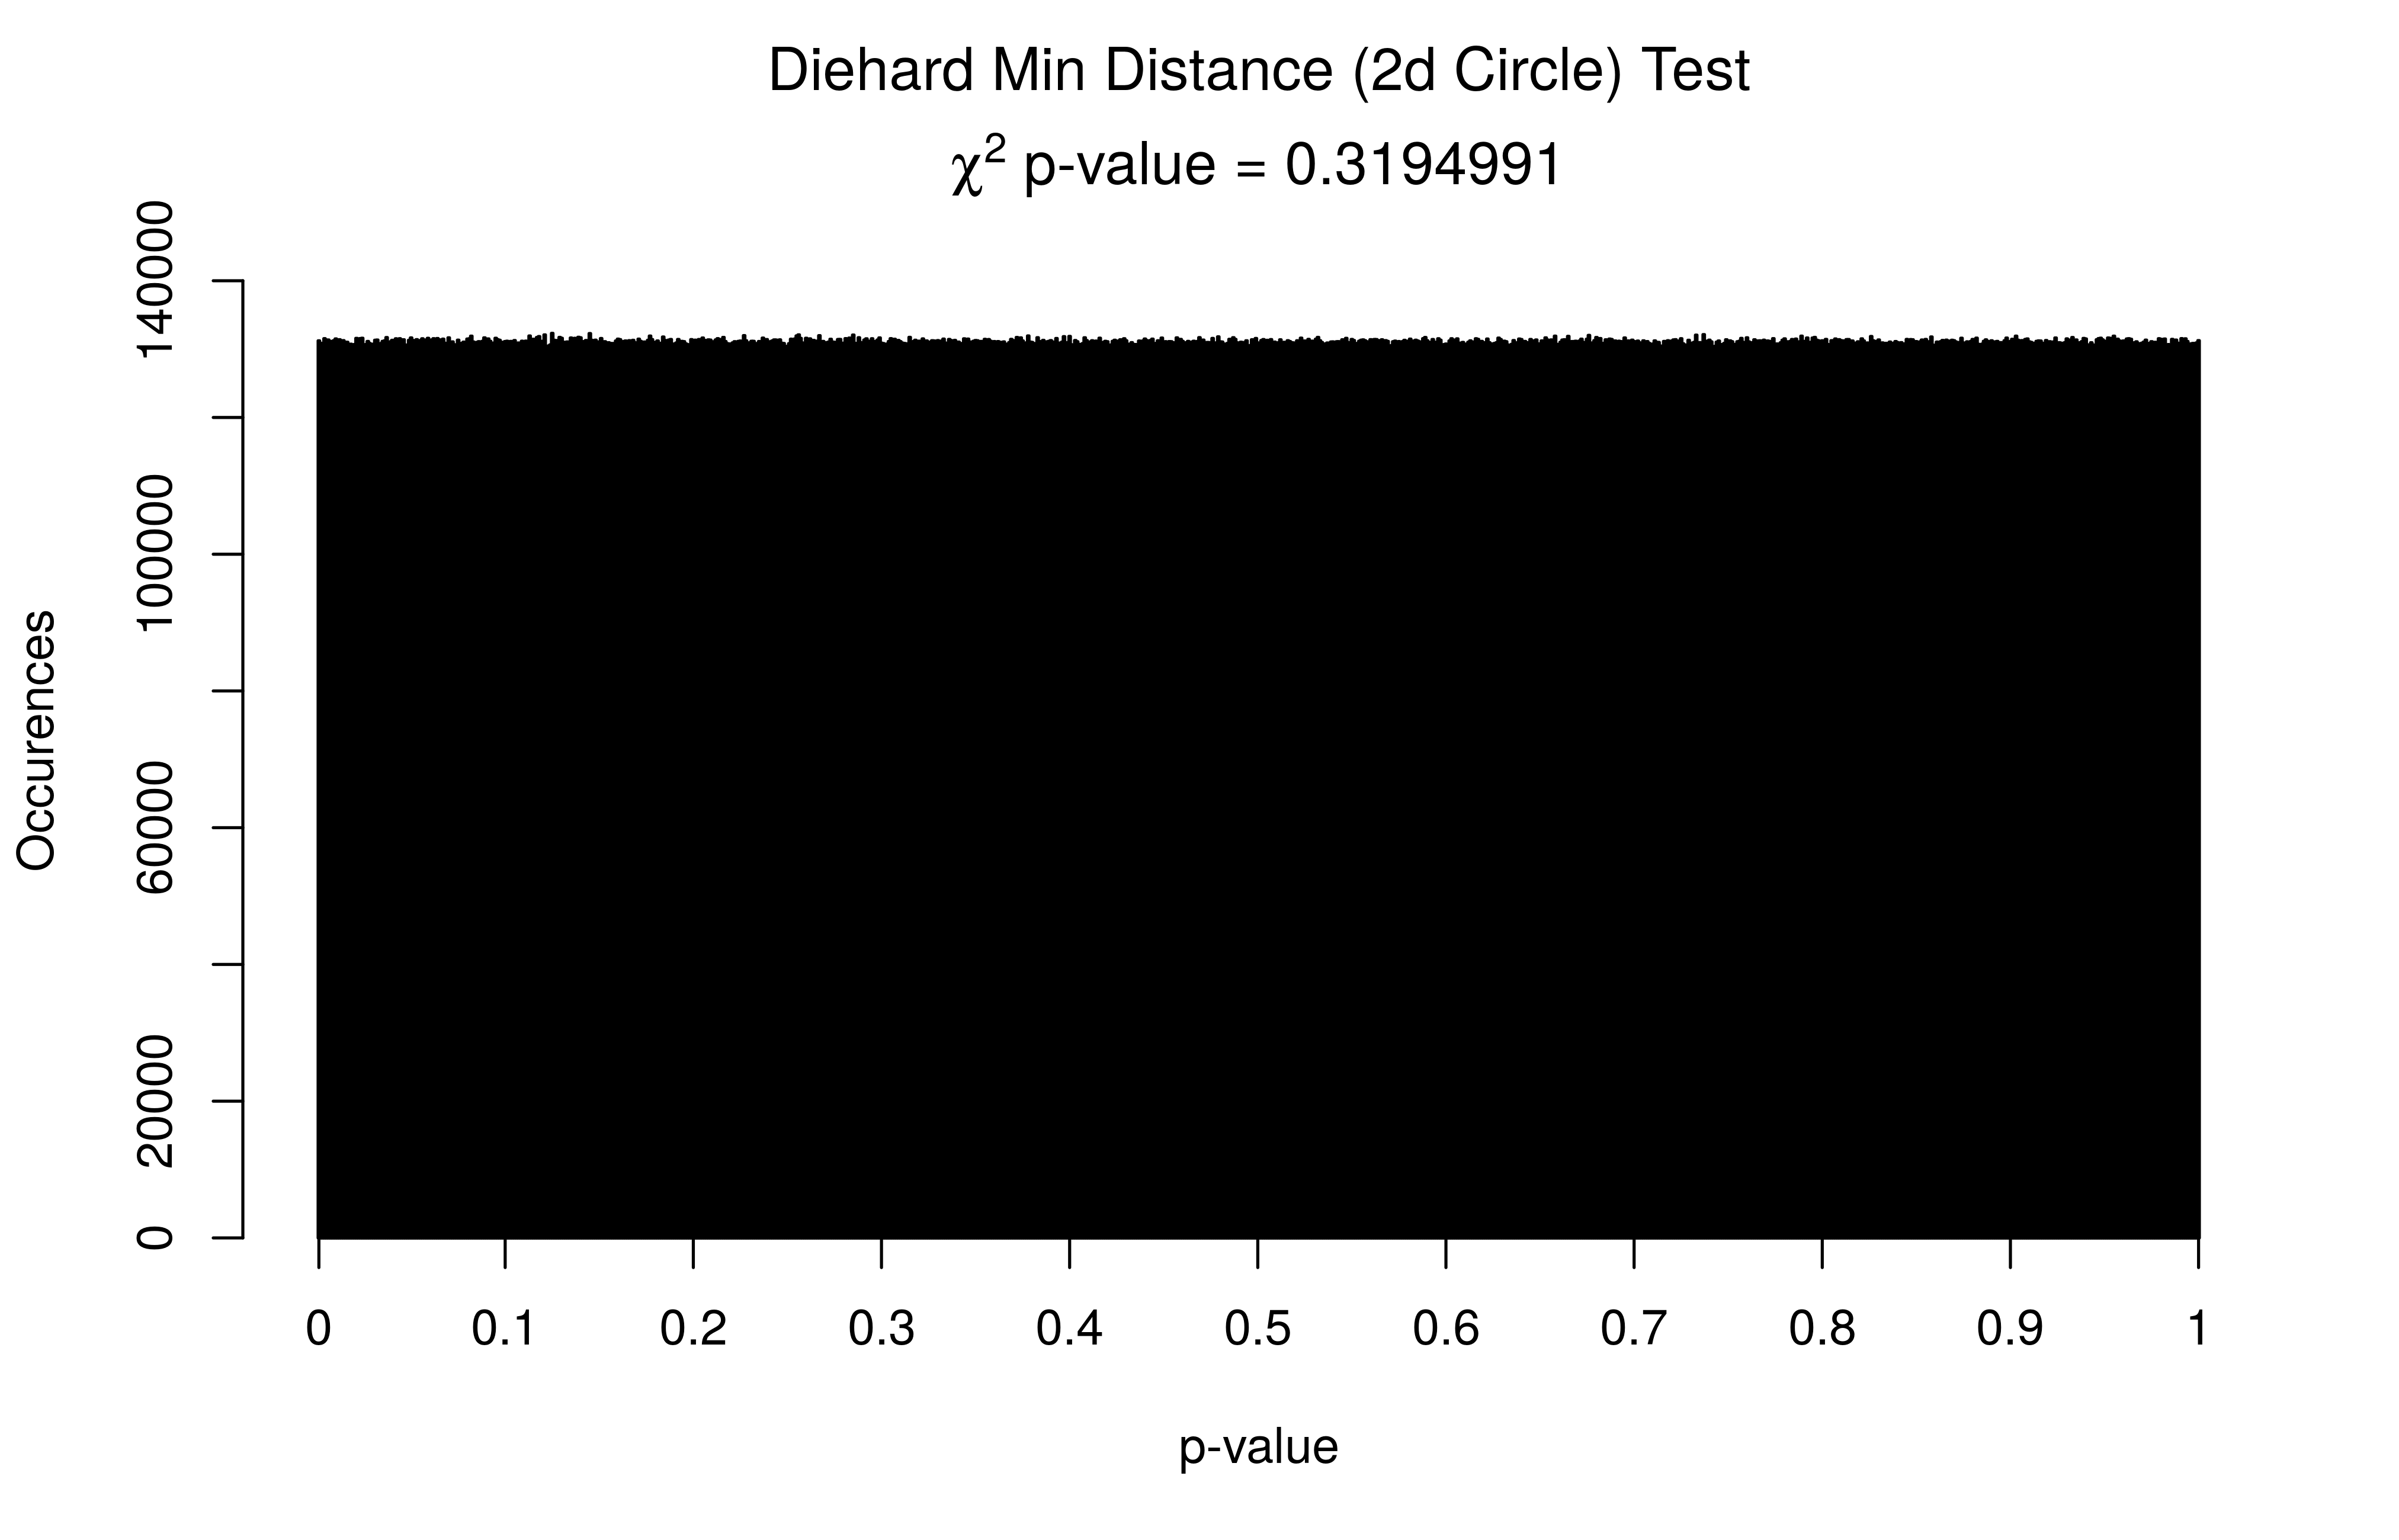
\includegraphics[width=.45\paperwidth]{figures/011.png} 
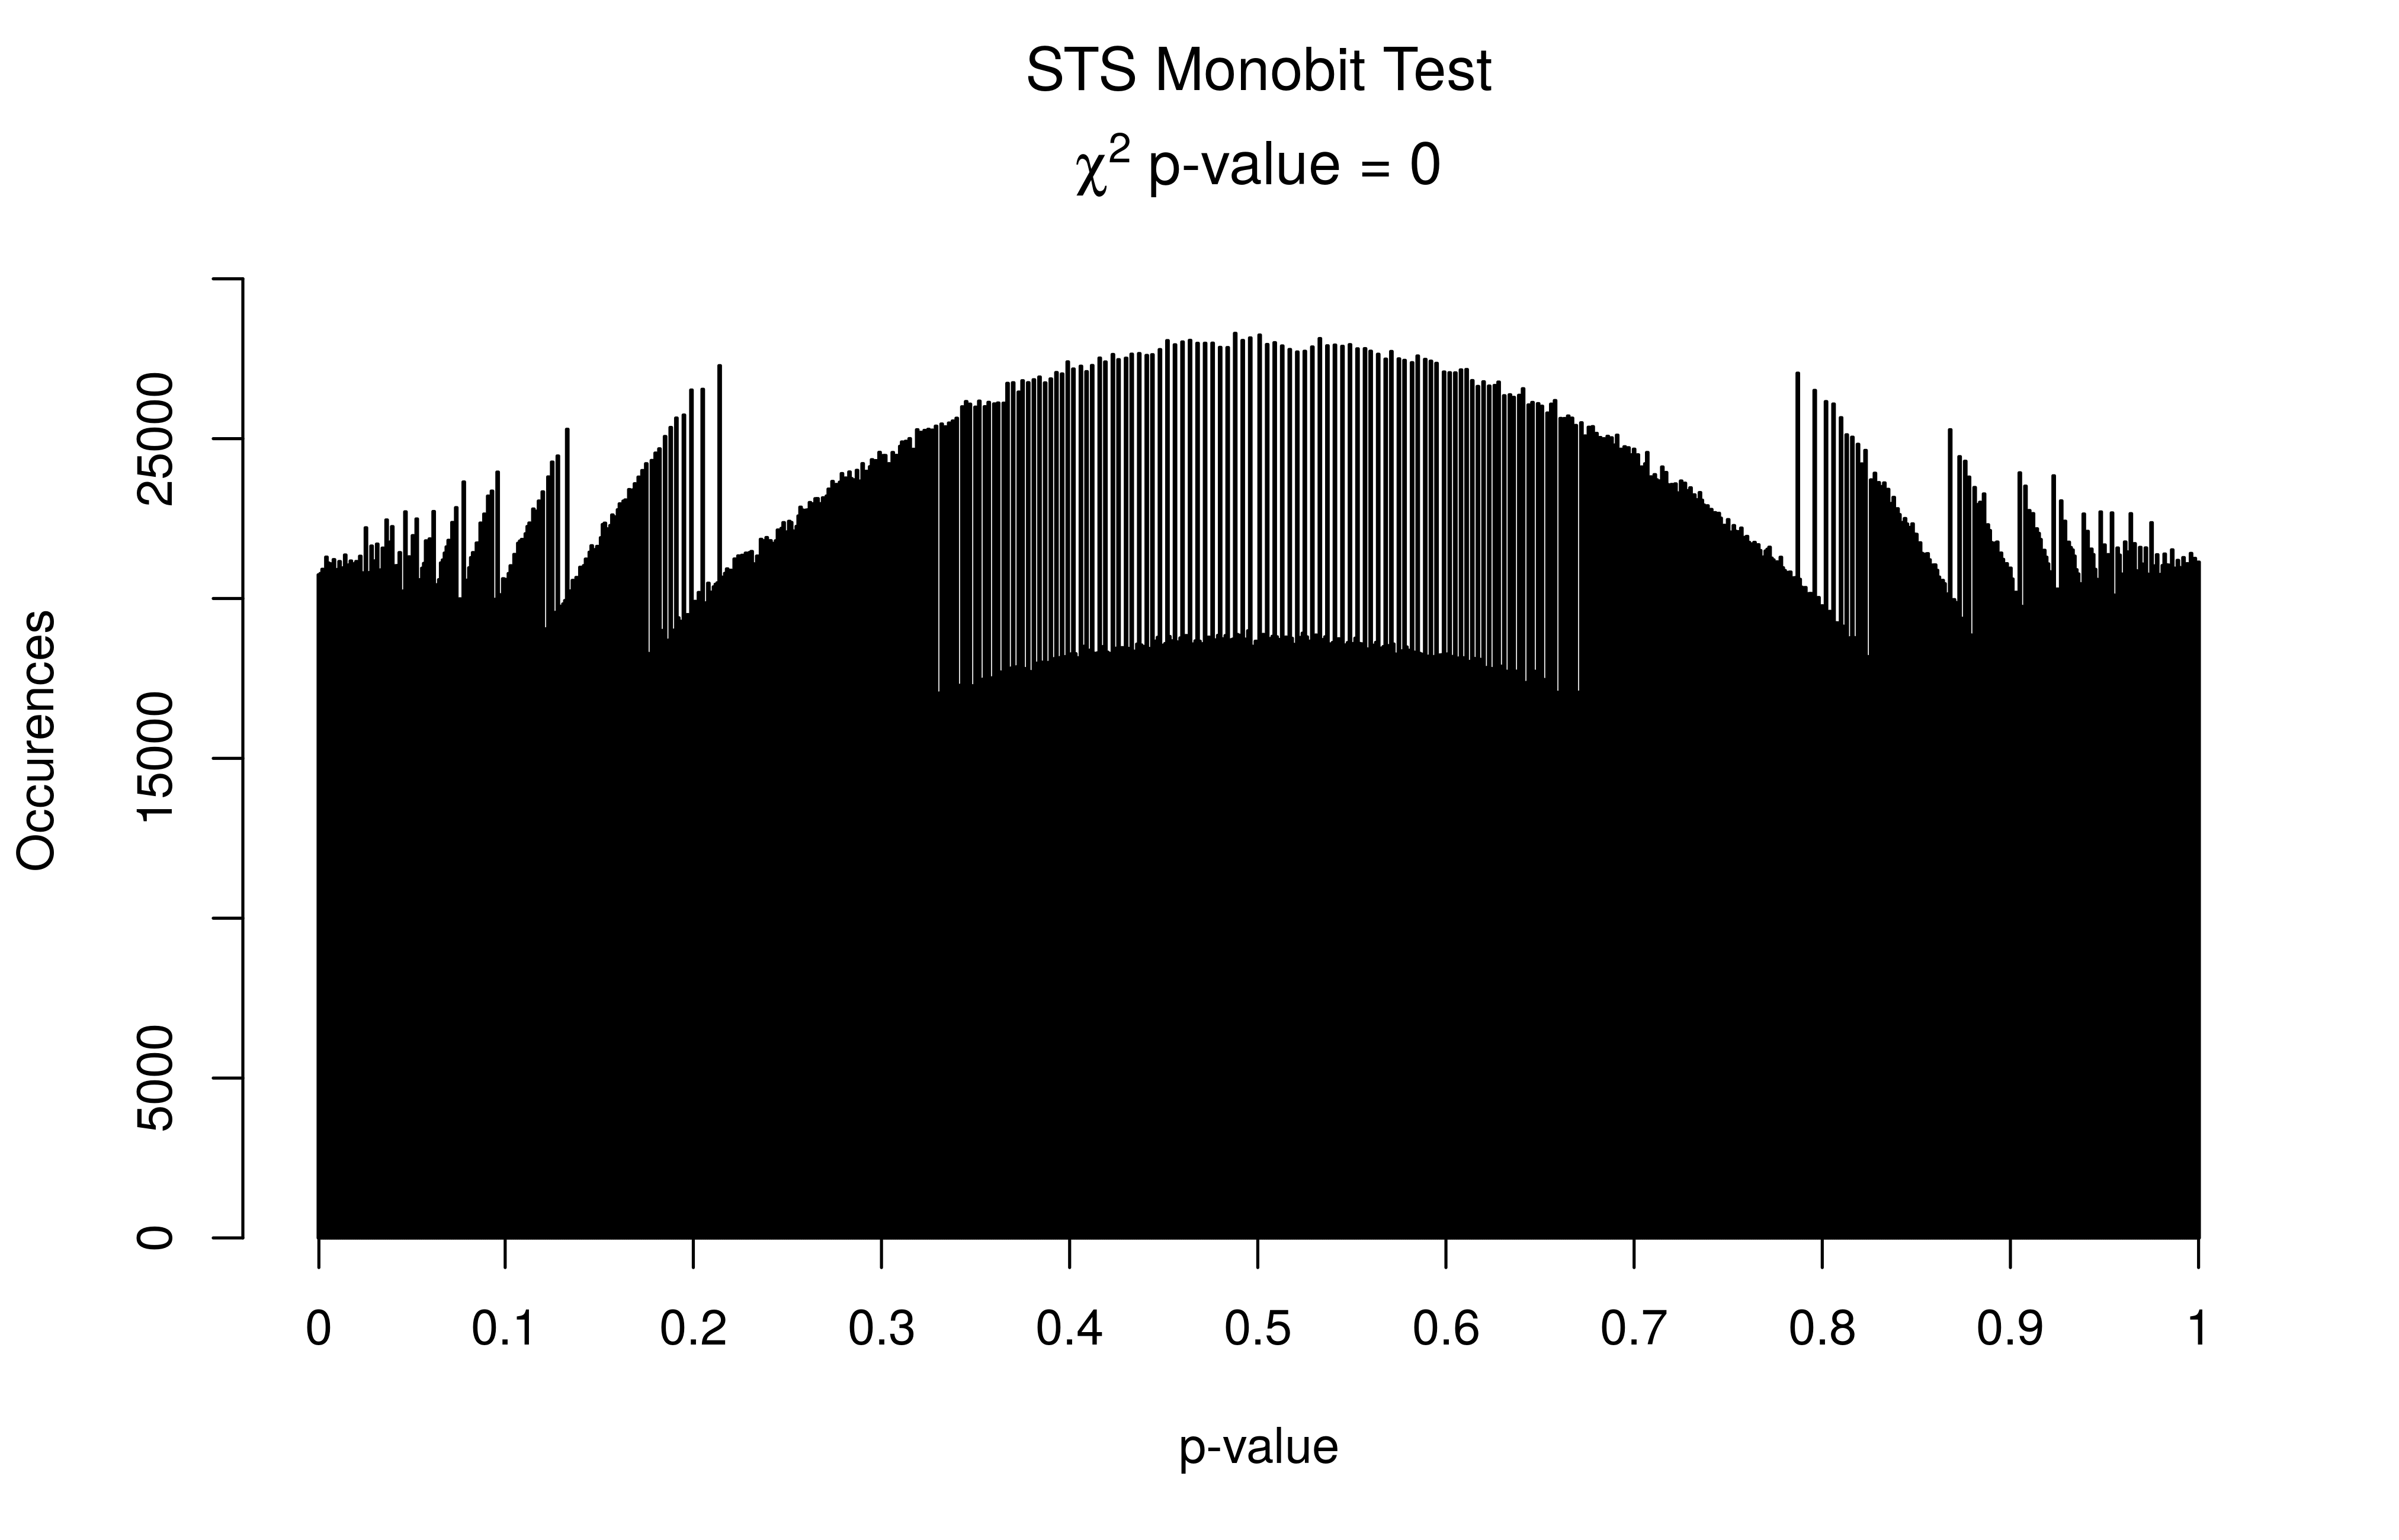
\includegraphics[width=.45\paperwidth]{figures/100.png}
\end{nomar}
\end{figure}

\end{frame}

\begin{frame}

\frametitle{References}
\begin{itemize}
\item \textbf{Randomness Testing Toolkit} \\ \url{https://github.com/crocs-muni/randomness-testing-toolkit}
\item \textbf{EACirc} \\ \url{https://github.com/crocs-muni/eacirc}
\item \textbf{NIST Statistical testing suite} \\ \url{http://csrc.nist.gov/groups/ST/toolkit/rng/documentation_software.html}
\item \textbf{Dieharder} \\ \url{http://www.phy.duke.edu/~rgb/General/dieharder.php}
\item \textbf{TestU01} \\ \url{http://simul.iro.umontreal.ca/testu01/tu01.html}
\end{itemize}

\end{frame}

\end{document}
